\chapter{Ontologies} \label{ch:ontologies}

\textbf{START here:} This is an easy story to tell if you walk through the
slides from your last committee meeting, and then answer any remaining
questions below.

*What is an ontology?

One important tool in understanding complex computing systems is an ontology.
An ontology captures knowledge by describing the classes, relationships
between, and entities of a system in formal way. 

*Ontology versus taxonomy

*Why do ontologies matter here?

*What does this look like in RDF?

*How can this be written in plain text, without invoking RDF?

\section{Case Study: A professor, a businessman, and a pilot}


\begin{figure}[htbp]
\centering
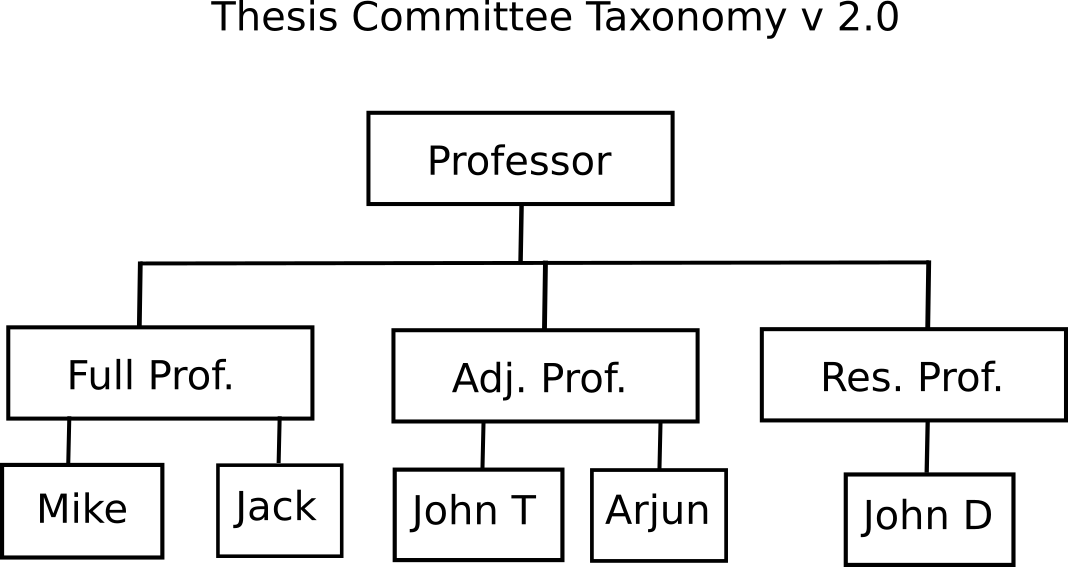
\includegraphics[width=\textwidth]{figures/tc-tax-v2.png}
\caption{Common data structures and their relationships in ICE.}
\label{data-arch}
\end{figure}

\begin{figure}[htbp]
\centering
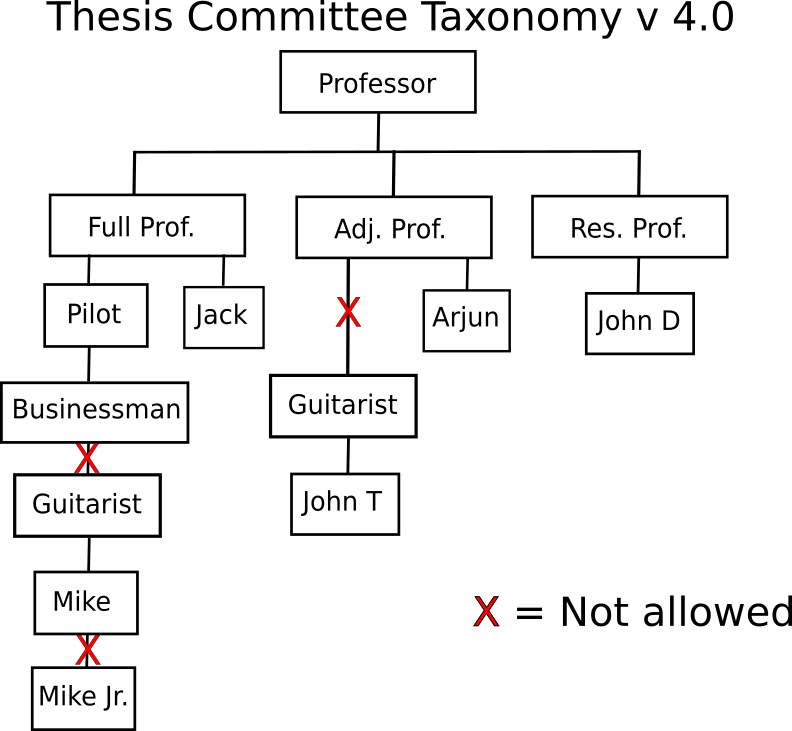
\includegraphics[width=\textwidth]{figures/tc-tax-v4-wErrors.png}
\caption{Common data structures and their relationships in ICE.}
\label{data-arch}
\end{figure}

\begin{figure}[htbp]
\centering
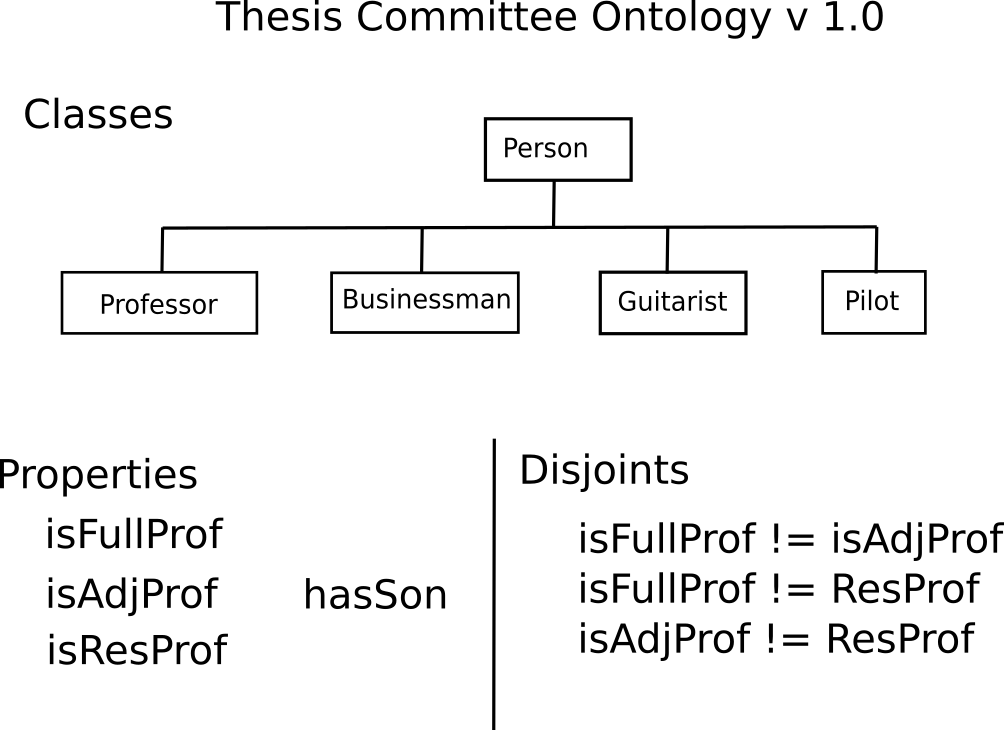
\includegraphics[width=\textwidth]{figures/tc-ont-classes.png}
\caption{Common data structures and their relationships in ICE.}
\label{data-arch}
\end{figure}

\begin{figure}[htbp]
\centering
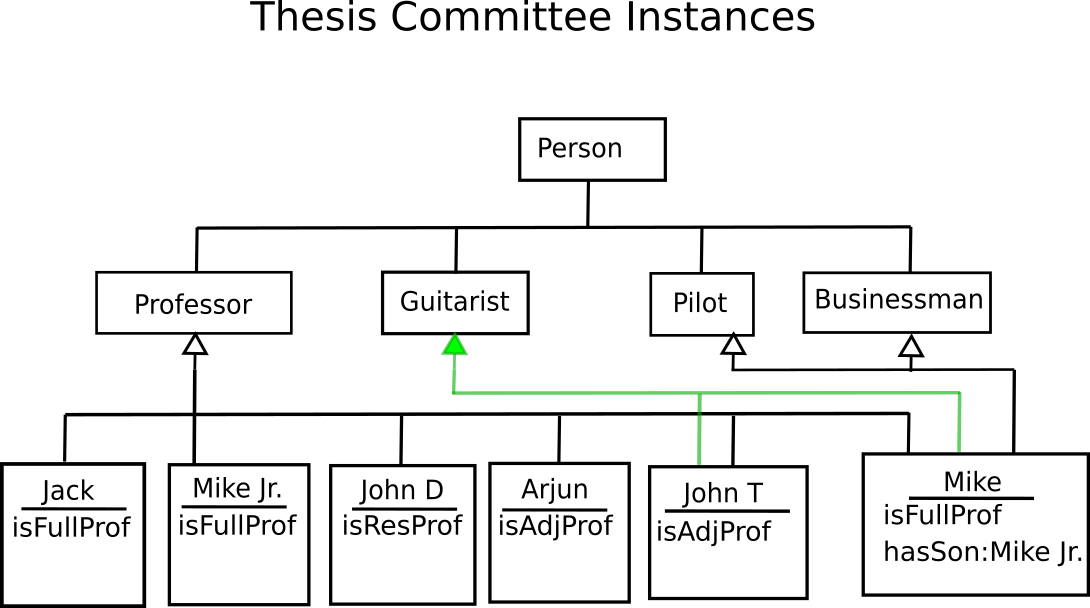
\includegraphics[width=\textwidth]{figures/tc-ont-instances.png}
\caption{Common data structures and their relationships in ICE.}
\label{data-arch}
\end{figure}


\section{The Resource Description Framework}

*What is RDF?

\subsection{RDF Schema (RDFS)}

\subsection{Web Ontology Language (OWL)}

\subsection{Our case study in RDF}

\section{A Workflow Ontology}

A workflow may be defined as a collection of tasks that are executed in some order by human and non-human actors. A workflow problem can then be defined as any problem that is solved the the execution of a specific workflow. Many systems exist that can execute workflows encoded in one or more \textit{description formats} for both business and scientific problems. There are predominantly three types of scientific workflows: High-throughput \cite{}, Modeling and Simulation \cite{}, and Analysis \cite{}.

Workflow problems of any of type can be decomposed into three required components: The workflow description, the \textit{workflow engine} that executes the workflow based on the description, and the data required to fully describe and execute the workflow. The latter may include - but does not necessarily require - metadata that describes the contents of the data itself, bulk data including values and quantities of interest used in the workflow. (For the purposes of this work, it is sufficient to consider provenance information as a type of metadata.)